\section{MCMC Hammer (nonlinear model)}

The data for this problem is the same as problem 5 therefore it can be described by the same Gaussian function described in equation \ref{eq:GaussModel}. 

For this problem we are going to use the MCMC Hammer method (emcee). 
The implementation of this method is describe in the previous problem by making the appropriate change in number of parameters and model difference. 

Figure \ref{fig:gaussEmcee} shows the posterior probability for this \\problem. 
As you can see, we practically get the same result as with the Metropolis-Hasting method. 
This also increases the confidence in that we are mapping the same posterior probability.  

The main advantage of emcee is takes a very small time in comparison with the Metropolis-Hastings me-thod.

% Repeat problem 5.7 using either the
% emcee package or by implementing your own slide-step sampler in place of the M-H sampler.
% Make sure you clearly describe both your implementation as well as what checks you do to make sure that things have worked well.

\begin{figure*}
    \centering
    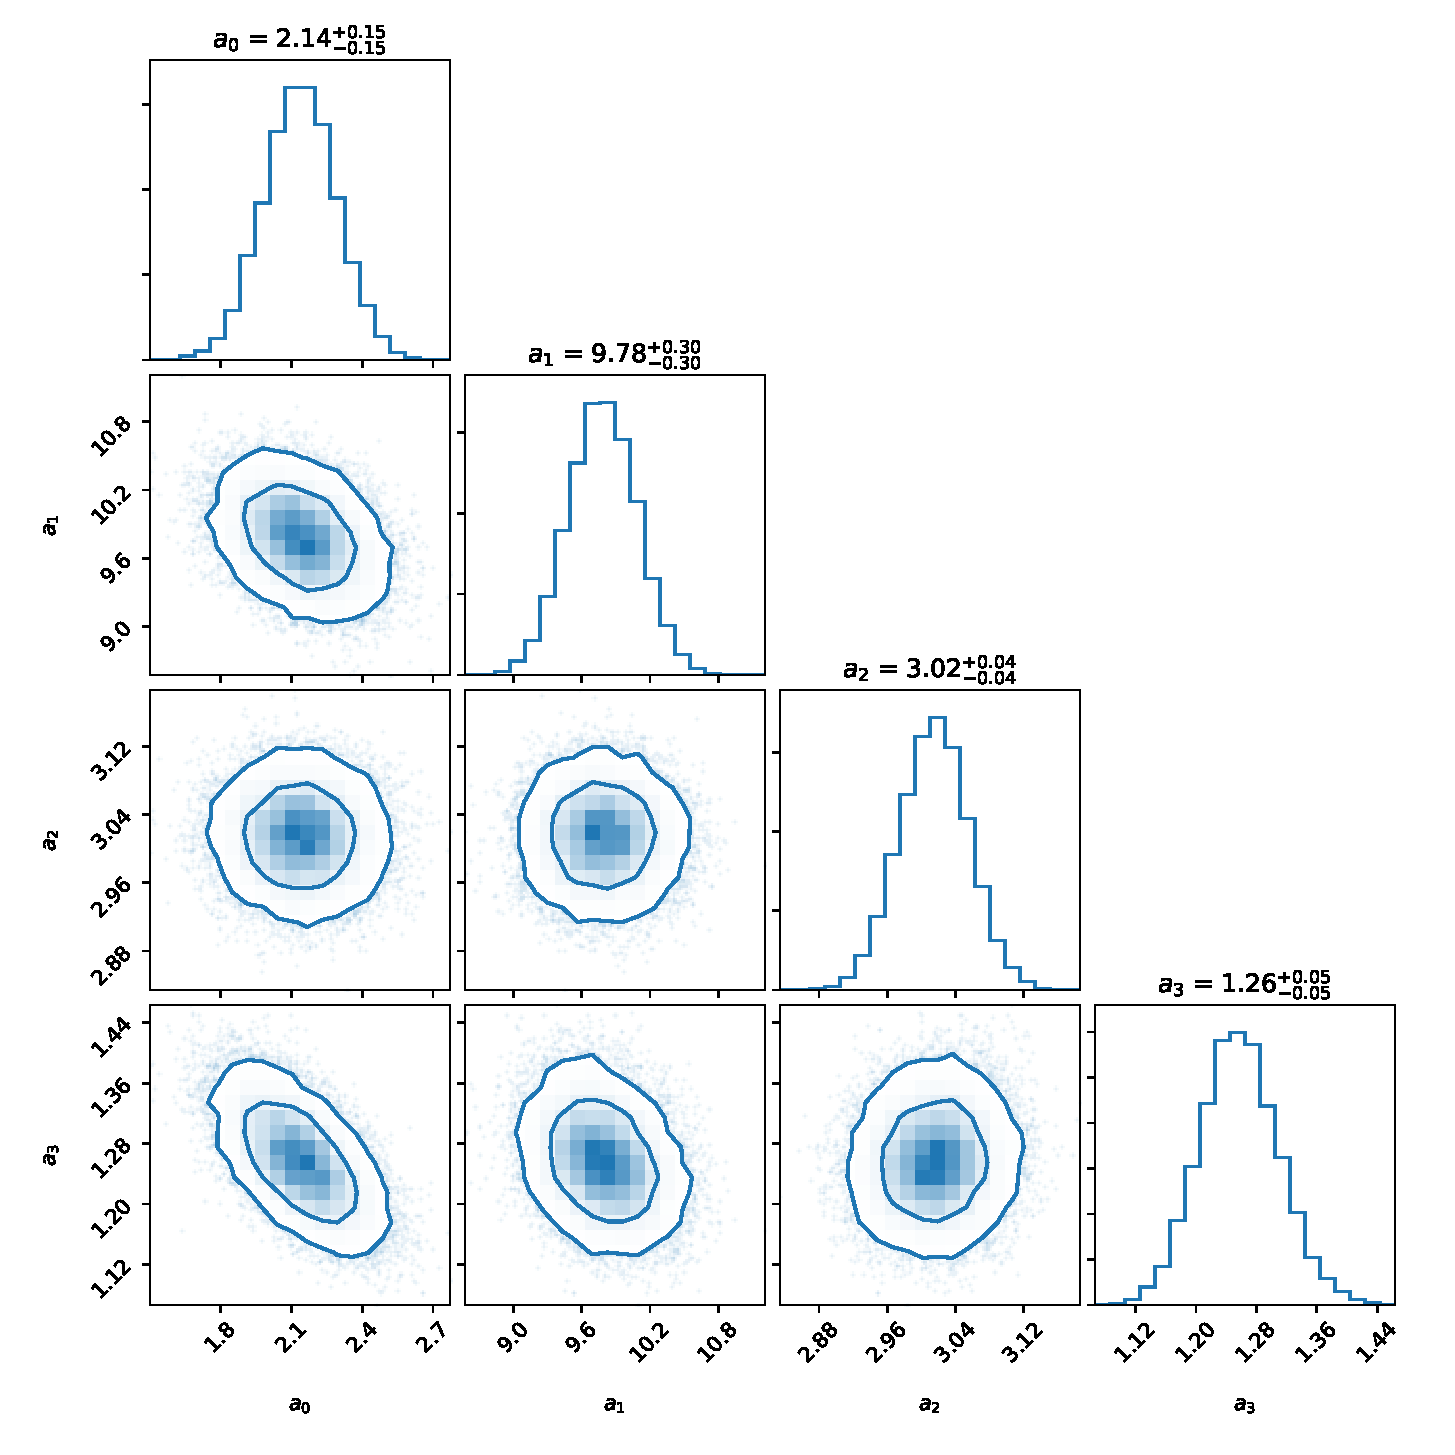
\includegraphics{CodeAndFigures/gaussianModelEmcee.pdf}
    \caption{Joint posterior probability distribution as well as the marginalized posterior probability of the data using the model described in equation \ref{eq:GaussModel} using MCMC Hammer method. The contours show the 68.3\% and 95\% confidence intervals.}
    \label{fig:gaussEmcee}
\end{figure*}